\chapter{Suppl\texorpdfstring{ementary}{.} material for Chap\texorpdfstring{ter}{.} \getrefnumber{ch:background}}%
\label{ch:SupplBack}

\section{Amino acids}\label{sec:aa}

As shown in \Cref{fig:aaformulas},
the amino acids have different chemical properties.
Their primary and side chains are respectively shown in black and green.
The amino acids all share the same primary chain.

\begin{figure}[htpb]
    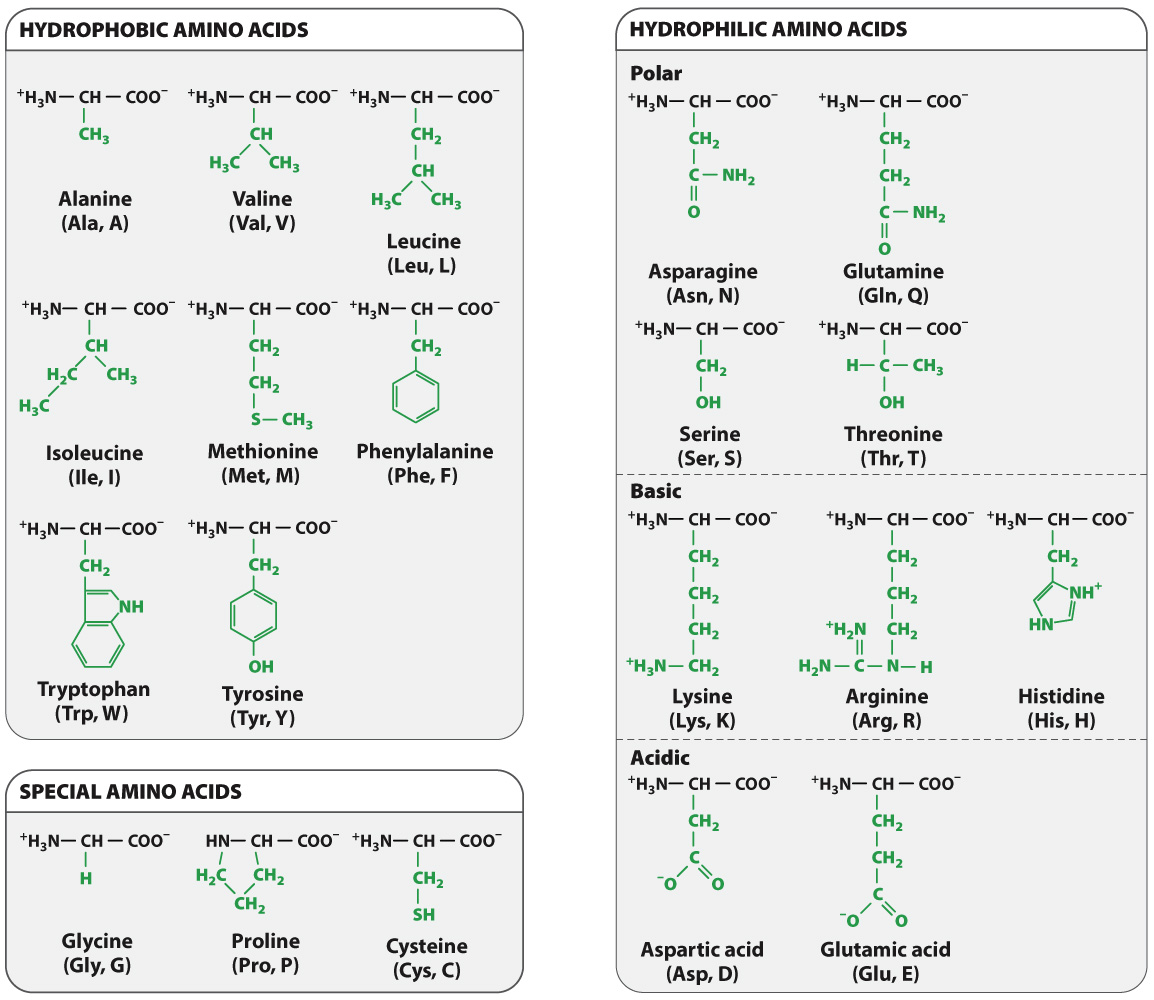
\includegraphics[scale=0.75]{background/aaformulas.jpg}\centering
    \caption[Amino acids formulas]{\label{fig:aaformulas}%
    \textbf{Amino acids formulas} --- from \citet{Morris2016-qv}}
\end{figure}


\begin{table}[]
\centering
\caption{Molecular weight of the most common \glspl{aa} and their residues}\label{tab:massAAs}
\begin{tabular}{@{}lllllll@{}}
\toprule
Name           & \multicolumn{2}{c}{Abbr.} & \begin{tabular}[c]{@{}c@{}}Molecular\\Formula\end{tabular} & \begin{tabular}[c]{@{}c@{}}Molecular\\Weight\end{tabular} & \begin{tabular}[c]{@{}c@{}}Residue\\Formula\end{tabular} & \begin{tabular}[c]{@{}c@{}}Residue Weight\\(-H2O)\end{tabular} \\ \midrule
Alanine & Ala & A & \ch{C3H7NO2} & 89.10 & \ch{C3H5NO} & 71.08 \\
Arginine & Arg & R & \ch{C6H14N4O2} & 174.20 & \ch{C6H12N4O} & 156.19 \\
Asparagine & Asn & N & \ch{C4H8N2O3} & 132.12 & \ch{C4H6N2O2} & 114.11 \\
Aspartic acid  & Asp & D & \ch{C4H7NO4} & 133.11 & \ch{C4H5NO3} & 115.09 \\
Cysteine & Cys & C & \ch{C3H7NO2S} & 121.16 & \ch{C3H5NOS} & 103.15 \\
Glutamic acid  & Glu & E & \ch{C5H9NO4} & 147.13 & \ch{C5H7NO3} & 129.12 \\
Glutamine & Gln & Q & \ch{C5H10N2O3} & 146.15 & \ch{C5H8N2O2} & 128.13 \\
Glycine & Gly & G & \ch{C2H5NO2} & 75.07 & \ch{C2H3NO} & 57.05 \\
Histidine & His & H & \ch{C6H9N3O2} & 155.16 & \ch{C6H7N3O} & 137.14 \\
Hydroxyproline & Hyp & O & \ch{C5H9NO3} & 131.13 & \ch{C5H7NO2} & 113.11 \\
Isoleucine & Ile & I & \ch{C6H13NO2} & 131.18 & \ch{C6H11NO} & 113.16 \\
Leucine & Leu & L & \ch{C6H13NO2} & 131.18 & \ch{C6H11NO} & 113.16 \\
Lysine & Lys & K & \ch{C6H14N2O2} & 146.19 & \ch{C6H12N2O} & 128.18 \\
Methionine & Met & M & \ch{C5H11NO2S} & 149.21 & \ch{C5H9NOS} & 131.20 \\
Phenylalanine & Phe & F & \ch{C9H11NO2} & 165.19 & \ch{C9H9NO} & 147.18 \\
Proline & Pro & P & \ch{C5H9NO2} & 115.13 & \ch{C5H7NO} & 97.12 \\
Pyroglutamatic & Glp & U & \ch{C5H7NO3} & 139.11 & \ch{C5H5NO2} & 121.09  \\
Serine & Ser & S & \ch{C3H7NO3} & 105.09 & \ch{C3H5NO2} & 87.08 \\
Threonine & Thr & T & \ch{C4H9NO3} & 119.12 & \ch{C4H7NO2} & 101.11 \\
Tryptophan & Trp & W & \ch{C11H12N2O2} & 204.23 & \ch{C11H10N2O} & 186.22 \\
Tyrosine & Tyr & Y & \ch{C9H11NO3} & 181.19 & \ch{C9H9NO2} & 163.18 \\
Valine & Val & V & \ch{C5H11NO2} & 117.15 & \ch{C5H9NO} & 99.13 \\ \bottomrule
\end{tabular}
\end{table}




\section{Original material}\label{sec:kelvinsong}
\vspace{-5mm}
To create \Cref{fig:transcriptionTranslation},
I used original material
by Kelvinsong (\href{https://commons.wikimedia.org/wiki/User:Kelvinsong}{https://commons.wikimedia.org/wiki/User:Kelvinsong}):
\enquote{Simplified diagram of mRNA synthesis and processing. Enzymes not shown.}
(\href{https://commons.wikimedia.org/wiki/File:MRNA.svg}{https://commons.wikimedia.org/wiki/File:MRNA.svg})
and
\enquote{Protein synthesis} (\href{https://commons.wikimedia.org/wiki/File:Protein\_synthesis.svg}%
{https://commons.wikimedia.org/wiki/File:Protein\_synthesis.svg}).

\vspace{-3mm}
\section[EST-sequencing]{Expressed~Sequence~Tag~(EST)~sequencing}\label{sec:EST}
\vspace{-5mm}
\glspl{EST} are short nucleotide sequence generated
from randomly selected \gls{RNA} transcript~\mycite{Parkinson2009-pj}.
\mRNAs\ are reverse transcribed into double-stranded \glspl{cDNA}
(either from the 5' or 3' end of the transcript)~\mycite{Lowe2017-kj}.
These \glspl{cDNA} are cloned to create libraries~\mycite{Harbers2008-qh}
and then sequenced either by Sanger method~\mycite{Sanger1975-io} or
a more high-throughput one such as
the sequencing-by-synthesis (\Cref{subsub:sequencing}).
Although this technique is subject to sampling bias~\mycite{EST} and
often account for only 60\% of an organism expressed genes~\mycite{Bonaldo1996-lx},
it remains a relatively low cost alternative approach to study the transcriptome
(gene discovery).


\vspace{-3mm}
\section{Microarrays}\label{sec:microarray}
\vspace{-5mm}
Microarrays require prior knowledge
(\eg\ annotated genome or \glspl{EST} libraries)
of the organism of interest
as they exploit it to design \emph{probes} (short nucleotide oligomers)
that are arrayed on a solid support (\eg\ a glass or silicon thin film cell)%
~\mycite{Lowe2017-kj,Schena1995-tg,Bumgarner2013-ey}.
For transcriptome profiling,
the expressed \glspl{RNA} are first reverse transcribed into \glspl{cDNA}
(also referred as \emph{targets})
and then, after being fluorescently labelled, they are complimentary hybridised
to the microarray probes;
the relative abundance of the transcripts is assessed
by measuring the intensity of the fluorescence
after the excess of unhybridised \glspl{cDNA} is washed away~\mycite{Lowe2017-kj}.
This technology is extremely powerful and popular
as it allows global and parallel analyses of cellular activity.
Microarray technology also has many variations~\mycite{Hoheisel2006-lw}
in addition to its original \gls{cDNA} version
for transcriptional profiling~\mycite{Schena1995-tg}, \eg\
for genotyping~\mycite{Wang1998-rs,Gunderson2006-pp},
protein profiling~\mycite{Hall2007-gt,Sutandy2013-tj,Duarte2017-ao},
splice-variant analysis~\mycite{Cuperlovic-Culf2006-rg} or
transcription factor binding~\mycite{Bulyk2002-ii,Bulyk2007-jc} studies.

\clearpage
\section{FASTQ format}\label{sec:fastq-format}

\begin{figure}[!htbp]
\begin{minipage}[adjusting]{\textwidth}
{\small
{\color[rgb]{0.447059,0.678431,0.274510}\verb!@ERR030856.1!}
{\color[rgb]{0.500000,0.500000,0.500000}\verb!HWI-BRUNOP16X_0001:1:1:2669:1073#0!}%
{\color[rgb]{1.000000,0.000000,0.000000}\verb!/1!}\\
\verb!AAAGGATTATGCAGANGTAGGGCGTGTNNNNNNNNNNNNNGGCTGGGGNNNNNNNNNNNNNNNNNNATNNNCTGACCANCTGAAGTATGTCANGCTGCCT!\\
{\color[rgb]{0.698039,0.145098,0.450980}+}\\
{\color[rgb]{0.000000,0.000000,0.555711}\verb!HHHHHHHIHHFFFFF#>>@>GGGFG###########################################################################!}\\
{\color[rgb]{0.447059,0.678431,0.274510}\verb!@ERR030856.2!}
{\color[rgb]{0.500000,0.500000,0.500000}\verb!HWI-BRUNOP16X_0001:1:1:4476:1072#0!}%
{\color[rgb]{1.000000,0.000000,0.000000}\verb!/1!}\\
\verb!GATAGATTATCAGAANGACAGTTACTTNNNNNNNNNNNNNGGGCACTTNNNNNNNNNNNNNNNNNNATNNNTCATAAGNNCTGTTGCCAAATNAGTGATA!\\
{\color[rgb]{0.698039,0.145098,0.450980}+}\\
{\color[rgb]{0.000000,0.000000,0.555711}\verb!HHHHHHHHHHDDDDD#@@AAGGGGG###########################################################################!}
}
{\footnotesize
Legend:\\
\quad{\color[rgb]{0.447059,0.678431,0.274510}\textbullet\ Read identifier}\\
\quad{\color[rgb]{0.500000,0.500000,0.500000}\textbullet\ Optional information (here flow cell lane:tile number:x:y:z)}\\
\quad{\color[rgb]{1.000000,0.000000,0.000000}\textbullet\ First member of pair (here) or single-end}\\
\quad\textbullet\ Nucleotide sequence of the read\\
\quad{\color[rgb]{0.698039,0.145098,0.450980}\textbullet\ Separator (+ or any string of character)}\\
\quad{\color[rgb]{0.000000,0.000000,0.555711}\textbullet\ Phred score (here Phred 33)}
}
\end{minipage}
\caption{FASTQ format}\label{fig:fastqFormat}
\end{figure}

\FloatBarrier\

\section{Phred score}\label{sec:PhredScore}

\begin{table}[!htbp]
\centering
\caption{Phred quality score to accuracy significance}%
\label{PhredtoAccuracy}
\begin{tabular}{@{}lll@{}}
\toprule
\begin{tabular}[c]{@{}l@{}}Phred quality\\ score ($Q$)\end{tabular} & \begin{tabular}[c]{@{}l@{}}Probability of\\ incorrect\\ base call\end{tabular} & \begin{tabular}[c]{@{}l@{}}Base call\\ accuracy\end{tabular} \\ \midrule
10 & 1 in 10 & 90\% \\
20 & 1 in 100 & 99\% \\
30 & 1 in 1,000 & 99.9\% \\
40 & 1 in 10,000 & 99.99\% \\ \bottomrule
\end{tabular}
\end{table}

The \gls{Phred} quality score can be encoded in several standards as shown in \Cref{phredformat}.
%https://en.wikipedia.org/wiki/FASTQ_format#Encoding
\begin{figure}[htbp]
\begin{minipage}[adjusting]{\textwidth}
\begin{verbatim}
SSSSSSSSSSSSSSSSSSSSSSSSSSSSSSSSSSSSSSSSS.....................................................
..........................XXXXXXXXXXXXXXXXXXXXXXXXXXXXXXXXXXXXXXXXXXXXXX......................
...............................IIIIIIIIIIIIIIIIIIIIIIIIIIIIIIIIIIIIIIIII......................
.................................JJJJJJJJJJJJJJJJJJJJJJJJJJJJJJJJJJJJJJJ......................
LLLLLLLLLLLLLLLLLLLLLLLLLLLLLLLLLLLLLLLLLL....................................................
!"#\$\%&'()*+,-./0123456789:;<=>?@ABCDEFGHIJKLMNOPQRSTUVWXYZ[\]^_`abcdefghijklmnopqrstuvwxyz{|}~
 |                         |    |        |                              |                     |
33                        59   64       73                            104                   126
 0........................26...31.......40
                          -5....0........9.............................40
                                0........9.............................40
                                   3.....9.............................40
 0........................26...31........41

S - Sanger        Phred+33, raw reads scores between  0 and 40
X - Solexa        Phred+64, raw reads scores between -5 and 40
I - Illumina 1.3+ Phred+64, raw reads scores between  0 and 40
J - Illumina 1.5+ Phred+64, raw reads scores between  3 and 40
        with 0=unused, 1=unused, 2=Read segment Quality Control Indicator
L - Illumina 1.8+ Phred+33, raw reads scores between  0 and 41
\end{verbatim}
\end{minipage}
\caption{The available Phred score quality score encoding formats}\label{phredformat}
\end{figure}

\begin{figure}[!htbp]
    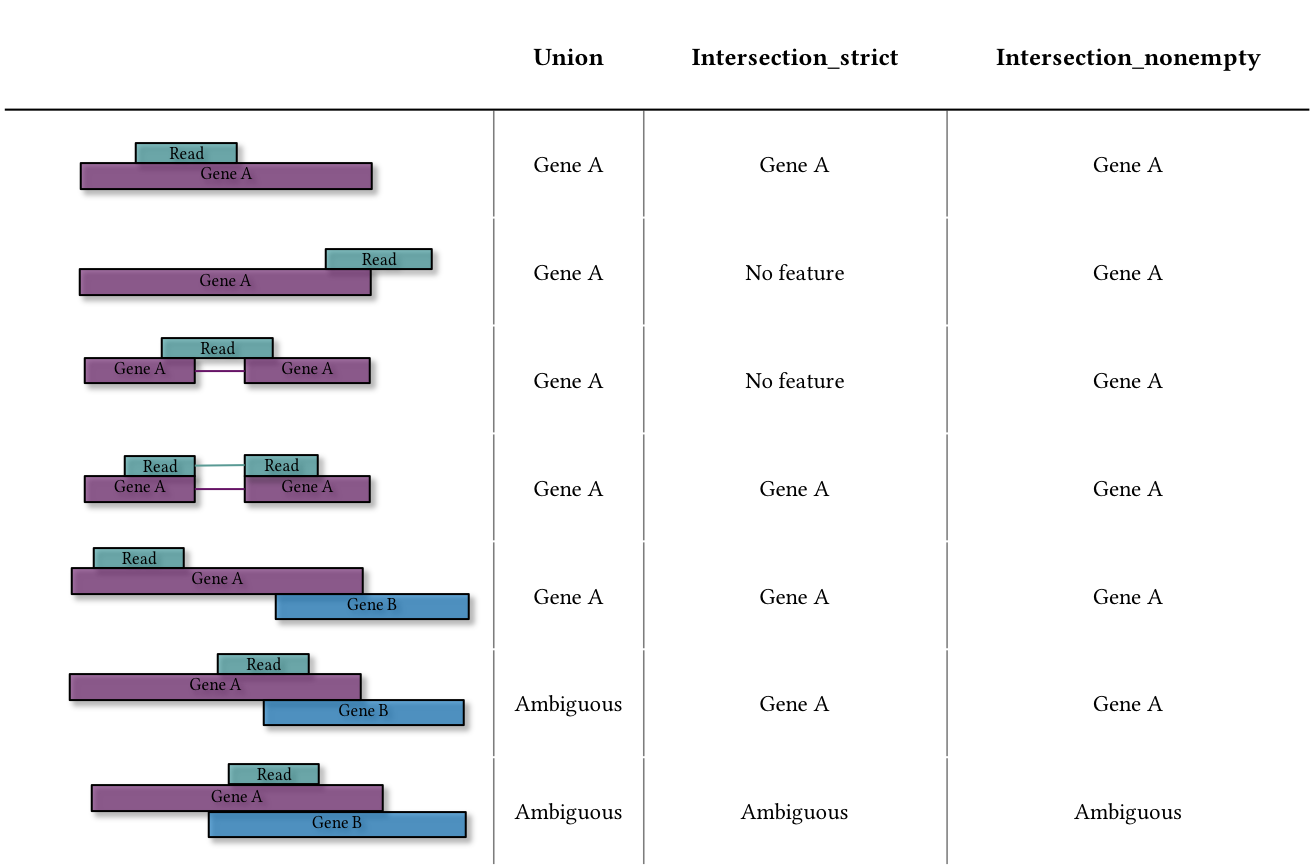
\includegraphics[scale=0.60]{background/interestHtseq}\centering
    \caption[Overlap resolution effects for each \htseq\
    mode]{\label{fig:htseqMode}\textbf{Overlap resolution effects for each \htseq\
    mode.} Each mode resolves a number of overlap situations differently. The
    mode used in this thesis is the \texttt{intersection non-empty} mode. This
    specific mode resolves more situations than the two others. Hence, the loss
    of ambiguous reads is reduced in this mode. [Adaptated from HTseq
    documentation: \footnotesize{\href{http://www-huber.embl.de/HTSeq/doc/count.html}%
    {http://www-huber.embl.de/HTSeq/doc/count.html}}]}
\end{figure}


\begin{table}[]
\centering
\caption{\gls{FPKM} are unsuitable for differential expression analysis}%
\label{tab:noFPKM4DEA}
\begin{tabular}{@{}lcccc@{}}
\toprule
\multicolumn{1}{l|}{} & \multicolumn{2}{c|}{Sample 1} & \multicolumn{2}{c}{Sample 2} \\ \midrule
\multicolumn{1}{l|}{} & \multicolumn{1}{c|}{raw counts} & \multicolumn{1}{c|}{normalised counts} & \multicolumn{1}{c|}{raw counts} & normalised counts \\ \midrule
\multicolumn{1}{l|}{$Gene_{1}$} & \multicolumn{1}{c|}{100} & \multicolumn{1}{c|}{0.010} & \multicolumn{1}{c|}{80} & 0.008 \\
\multicolumn{1}{l|}{$Gene_{2}$} & \multicolumn{1}{c|}{100} & \multicolumn{1}{c|}{0.010} & \multicolumn{1}{c|}{80} & 0.008 \\
\multicolumn{1}{c}{\ldots} & \ldots & \ldots & \ldots & \ldots \\
\multicolumn{1}{l|}{$Gene_{i}$} & \multicolumn{1}{c|}{100} & \multicolumn{1}{c|}{0.010} & \multicolumn{1}{c|}{80} & 0.008 \\
\multicolumn{1}{l|}{$Gene_{i+1}$} & \multicolumn{1}{c|}{0} & \multicolumn{1}{c|}{0} & \multicolumn{1}{c|}{2000} & 0.2 \\ \midrule
\begin{tabular}[c]{@{}l@{}}Total number\\ of fragments ($F$)\end{tabular} & 10,000 & 1 & 10,000 & 1 \\ \bottomrule
\end{tabular}
\end{table}

\FloatBarrier\


\section{Mass analysers}\label{sec:appMassAnalysers}

See~\citet{Haag2016} for more details on other types of analysers.

\minisec{Quadrupole analyser}
It is one of the most popular analysers as they are cheap compared to the
others. They are also compact, durable and reliable. The quadrupole analyser can
filter the ions based on their difference of $m/z$. They are adequately
named quadrupole as they comprise four cylindrical or hyperbolic rods in
parallel to each other. Opposite rods are connected together electrically and
\gls{RF} potential is applied. A \gls{DC} potential is superimposed on the
\gls{RF} one. These combinations of \gls{RF} and \gls{DC} potentials constrain the
ions to oscillate between the rods as they pass through them. Hence, by tuning
the \gls{RF} and \gls{DC}, it is easy to select for which range of $m/z$ ions
will have a stable trajectory and thus the only one detected. Indeed, the
ions with unstable trajectory will collide with the rods and be \enquote{filtered}
out. If used in \enquote{\gls{RF}-only} mode (\gls{DC} reduced to a minimum),
the quadrupole may have other applications. For example, it can guide specific
$m/z$ ions to other areas (while the bulk of ions will remain trapped).
It may also be used as collision cells for \gls{CID}: by introducing an inert
gas and tuning with the \gls{RF}-energy, the amount of fragmentation undergone
by the targeted ions can be precisely controlled. \mycite{Haag2016}\\
The quadrupole analyser is also qualified as the \emph{mass filter}.

\minisec{\Acrfull{LTQ}}
\gls{LTQ} is a particular kind of \acrfull{LIT} which is in principle a sort of
a quadrupole mass analyser~\mycite{Zhang2014}. A \gls{LTQ} uses a set of
quadrupole rods and a two-dimensional \gls{RF} field confines the ions radially.
In addition, a static electrical potential is applied to end electrodes which
forbid the ions to escape axially. However, the quadrupole is commonly segmented
into three parts which ensure a perfect homogeneity of the electric field of the
trap area and thus avoiding ion loss when the trapping is done.
While they may be used as an ion trap, they
may be also used as a simple mass filter. \gls{RF} voltage is tuned to produce
multi-frequency resonance ejection waveforms are applied as to
eliminate all the undesirable ions in the trap before the fragmentation and mass
analysis of the remaining ones. Frequently, these \glspl{LTQ} are used as a
front-end to other mass analysers as they have high injection efficiencies and
high ion storage capacities. They may be equipped then with two biased radial
ejection slits and then be used with two detectors hence the signal-to-noise
ratio may be doubled.

Compared with other traps, linear ion traps provide an enhanced dynamic range
with a reduced low mass cut-off as the ion cloud is
spatially distributed on a linear axis and not a 3D centre which improves the
sensitivity. And then, for example, the ions may then be accumulated before
being released into another mass analyser~\mycite{Madalinski2008}.

\minisec{\orbi}
It is a very recent analyser and it relies on \gls{FT}. Recently,
there is increasing use of \glspl{FTMS} for proteomic studies. Indeed, these
\glspl{FTMS} are more precise than previous analysers and allow the detection of
a greater range of ions in very short lapses of time~\mycite{Scigelova2011}.
In this kind of analyser, ions are trapped and both orbit around and oscillate
in an electrostatic field between an inner and outer part of a central electrode
shaped as a spindle.
The ions can only move following the spindle long axis~\mycite{Makarov2000}.
While moving around the spindle the ions create a current.
The outer part of the spindle records images of this current.
Fourier transformation of these images allows obtaining very highly accurate
and sensitive mass spectra for a greater dynamic range than most of the
other analysers.~\mycite{Hu2005}

\minisec{\gls{LTQ}-\orbi}
It is a hybrid (tandem) mass spectrometer that uses \gls{ESI} for the ionisation
step and has an \gls{LTQ} as a first analyser (MS$^1$)
and an \orbi\ as a second one (MS$^2$).
This \gls{MS/MS} enables multiple levels of
fragmentation for the elucidation of a wide range of peptides and can be coupled
with an \gls{ESI} which is a continuous source of ionisation. This instrument
allows analysing proteomic samples optimally both in terms of starting material,
time~\mycite{Scigelova2011} and provides \enquote{ultrahigh} mass resolution,
high mass accuracy
and enhanced dynamic range with respect to mass accuracy~\mycite{Madalinski2008}.

\section{Isotopes of common elements and their natural
frequency}\label{app:isotopes}
\Cref{tab:isotope} lists the mass~\mycite{Audi1993-qn,Audi1995-uk}
and the percent natural abundance~\mycite{Rosman1998-xu}
for stable nuclides (\ie\ atom distinctly characterised by its number of protons (Z)
and number of neutrons (N)) that may be found in \glspl{DNA}, \glspl{RNA} and proteins.

\begin{table}[!htbp]
\centering
\caption[Most common elements and their stable isotopes]%
{\textbf{Most common constitutive elements and their stable isotopes\\ found in DNAs,
RNAs and proteins.} Asterisks (*) mark abundances that are not available.
Adapted from~\mycite{Audi1993-qn,Audi1995-uk,Rosman1998-xu}
}%
\label{tab:isotope}
\begin{tabular}{@{}clccr@{}}
\toprule
\begin{tabular}[c]{@{}c@{}}%
    z \\ (Atomic number)\end{tabular} &
    \multicolumn{1}{c}{Name} & Isotope &
    \begin{tabular}[c]{@{}c@{}}Mass atomic\\ (u)\end{tabular} &
        \multicolumn{1}{c}{\begin{tabular}[c]{@{}c@{}}Natural frequency\\ (\%)\end{tabular}} \\
\midrule
1  & Hydrogen & \isotope[1]{H} & 1.007825 & 99.9885 \\
   & Deuterium & \isotope[2]{H} & 2.014102 & 0.0115 \\
   & Tritium & \isotope[3]{H} & 3.016049 & * \\
6  & Carbon & \isotope[12]{C} & 12.000000 & 98.93 \\
   &  & \isotope[13]{C} & 13.003355 & 1.07 \\
   &  & \isotope[14]{C} & 14.003242 & * \\
7  & Nitrogen & \isotope[14]{N} & 14.003074 & 99.632 \\
   &  & \isotope[15]{N} & 15.000109 & 0.368 \\
8  & Oxygen & \isotope[16]{0} & 15.994915 & 99.757 \\
   &  & \isotope[17]{0} & 16.999132 & 0.038 \\
   &  & \isotope[18]{0} & 17.999160 & 0.205 \\
15 & Phosphorus & \isotope[31]{P} & 30.973762 & 100 \\
16 & Sulphur & \isotope[32]{S} & 31.972071 & 94.93 \\
   &  & \isotope[33]{S} & 32.971458 & 0.76 \\
   &  & \isotope[34]{S} & 33.967867 & 4.29 \\
   &  & \isotope[35]{S} & 35.967081 & 0.02 \\
53 & Iodine & \isotope[127]{I} & 126.904468 & 100 \\
\bottomrule
\end{tabular}
\end{table}

\section{Hypothesis testing}\label{pq-values}

\subsection{$\mathcal{H}_0$}\label{H0}
In statistical testing,
the null hypothesis $\mathcal{H}_0$ is an answer
to the intrinsic nature of statistical calculation:
the smaller a given interval is,
the lower the probability of a simple random draw in that interval.
The null hypothesis can be of different natures.
It is generally formulated as an absence of difference
between two objects to be compared,
or as an absence of relationship between two variables of a same population;
its purpose is to be rejected.
It is always opposed to another \emph{alternative} hypothesis ($\mathcal{H}_1$),
which is accepted when $\mathcal{H}_0$ is rejected.

To test an hypothesis,
one needs to construct a statistical model that can represent an ideal form
of the data if it were to be generated by random processes alone.
This model is also referred as the \emph{distribution under the null hypothesis}.
Then, the likelihood of the collected (observed) data is computed.
Finally, it is compared to the (random) probability determined by the model
to either accept $\mathcal{H}_0$ or reject it
if the observed data is very unlikely under the null hypothesis.
Usually a test statistic
(\ie\ quantity derived from the sample used for the hypothesis testing)
that measures the apparent departure from the null hypothesis is compared
to a value defined such as the probability of a \enquote{more extreme value}
is even smaller under the null hypothesis.
Prior to the analysis, an arbitrary level of significance (or $\alpha$) is
set either to 0.1, 0.05, 0.01, 0.005 or 0.001,
\ie\ 10\%, 5\%, 1\%, 0.5\% or 0.1\% risk to reject $\mathcal{H}_0$ by mistake.

Depending on whether the observed data is tested, case (1): in both direction,
\ie\ the data is either \emph{greater or equal} to the critical value ($x$) or
\emph{lesser or equal} to the additive inverse of the critical value ($-x$),
or, case (2) in one direction only,
\ie, (for example) the data is (only) \emph{greater or equal} to the critical value
(or the data is (only) \emph{lesser or equal} to the critical value),
the statistical test is two-tailed (case 1) or one-tailed.

\subsection{p-value}\label{p-value}
In statistical hypothesis testing,
the p-value quantifies the statistical significance of results,
under the null hypothesis $\mathcal{H}_0$ (see \Cref{H0}).
It allows rejecting (or not) $\mathcal{H}_0$.
The p-value is the probability for a given statistical model of obtaining
an equal value or an even more extreme value than what has been observed
when $\mathcal{H}_0$ is true.
Depending on the situation,
the more extreme value can mean:
\begin{eqlist}
        \item[One-tail event]
            \begin{eqlist}
            \item[Left tail event]  $\text{Pr}(X \leq x \mid \mathcal{H}_0)$
            \item[Right tail event] $\text{Pr}(X \geq x \mid \mathcal{H}_0)$
            \end{eqlist}
        \item[Two-tail event] $2\text{min}(\text{Pr}(X \leq x \mid \mathcal{H}_0),%
            \text{Pr}(X \geq x \mid \mathcal{H}_0))$
\end{eqlist}
The smaller is a p-value,
the higher the significance, \ie\
the stronger the evidence that $\mathcal{H}_0$ has to be rejected.
$\mathcal{H}_0$ is rejected if the adequate probability is less than or equal to
an arbitrary pre-defined (\ie\ prior to the analysis) threshold value $\alpha$.

Under $\mathcal{H}_0$,
the assumption is that the p-values are uniformly distributed.\mybr\

\subsection{q-value}\label{q-value}\label{multitesting}
A q-value is an adjusted p-value
(which the calculation may or may not be based on the p-value).
In the context of multi-testing,
\ie\ when multiple simultaneous statistical tests occur,
the likelihood of rejecting $\mathcal{H}_0$ due to a random sampling increases.
To avoid accepting the alternative hypothesis by mistake,
the whole p-values collection is tested and adjusted for \glsentrydesc{FDR}.
A q-value of 5\% means that 5\% of all the significant results
are actually false positives.

\section{Target Decoy search database}\label{app:tda}
For best effectiveness,
decoy and target peptide sequence databases are searched with the same parameters.
Furthermore, to ensure that
a wrong hit in the target database and a hit in the decoy one are equally likely,
the decoy sequences have to be as similar as possible to the target ones
(concerning \gls{aa} frequencies and composition,
length, mass, charges, assigned scores).
There are different ways to design the decoy sequences.
For example, by reversing the peptide or protein sequences,
either with complete or pseudo-reversion (where the last \gls{aa} is kept in place).
Alternatively, by using stochastic methods on the target database
such as the randomisation of the sequences or
through the creation of new ones based on \gls{aa} frequencies,
their length distribution,
and their number in the original database;
Markov models~\mycite{Gagniuc2017-nj} are often used
to mimic the closest target sequences.
Many studies explore and compare the different decoy creation
methods~\mycite{Elias2007-wi,Wang2009-ww,Elias2010-kp,Wright2016-as}.
As for the target database,
the decoy sequences are digested \latin{in silico} before the search.
While the search can be done independently
on the target and the decoy databases~\mycite{Blanco2009-u6},
\citet*{Elias2007-wi} report that
searching their resulting concatenation gives better results.\mybr\

Besides, the \gls{TDA} approach can guide
the selection of sensitive \psm\ attributes
(\eg, elution time, charge, peptide length, score)
as filtering criteria to discern correct identifications~\mycite{Elias2010-kp}.

\section{PSM validation with q-value and PEP}\label{app:qvalPEP}

A possible definition of \psm's \emph{q-value}\label{qvalP} is
the minimal \gls{FDR} threshold for which the \psm\ is accepted as correct.
As the q-values are derived from the \gls{FDR},
which is specific to a \psm\ collection,
they are also (solely) specific to this collection.
For example,
\soft{Percolator} estimates the q-value
by using the score distribution from the \gls{TDA}.
On the other hand,
\glsentrydesc{PEP} (\gls{PEP})\label{PEP}
(also known as \emph{local \gls{FDR}}~\mycite{Efron2001-ai})
is the probability of a \psm\ being incorrect;
a \psm's \gls{PEP} is independent of the \psm\ collection.
A classical approach to estimating \glspl{PEP} uses
training sets of target and decoy \psms\ to learn the parameters
of a probability model (indispensable to compute the \glspl{PEP}).
Thus, for each given score (of any collection), a specific \gls{PEP} is associated.
\citet{Choi2008-ec} showed that for a given collection,
the sum of the \glspl{PEP} is equal to the expected number of incorrect \psms,
which allows calculating the (global) \gls{FDR}.\mybr\

\section{Protein~inference:~computational~challenging~step}\label{app:inferenceChallenge}

To explain the computational challenges of the peptide assembly,
\citet{Huang2012-nr} propose to start with two assumptions:
(1) all ($m$) peptides are true positive,
and (2) peptides have an equal probability of detectability.
A first assumption corollary is
the presence of many homologous proteins in the sample.\mybr\

Besides, one can derive from the first assumption
that there are a minimal and a maximal value
for the number $n$ of proteins that can be identified
from the set of $m$ peptides.
Returning the exhaustive list of proteins (\ie\ $n_\text{Max}$)
that comprise all $m$ peptides (\eg\ \citet{Tabb2002-wm}) is one possible solution,
but it is much more difficult to calculate the minimal list
(\ie\ $n_\text{min}$) that does the same.
As all the peptides $m$ are supposed to be true,
they have to be included in any of the final minimal list proteins.
Therefore inferring this protein list can be formulated
as a \emph{set covering problem}~\mycite{Cormen2009-rk,Hochbaum1997-db}.
The set covering problem is known to be \gls{NP}-complete~\mycite{Van_Leeuwen1990-sn},
and for which it is in practice impossible to calculate an optimal solution.
Usually, algorithms approximate this solution through a parsimonious approach.\mybr\

Many inference algorithms seek
a compromise between the minimal and exhaustive lists of possible proteins.
While the minimal list probably excludes many true positives
(but can still include false positives),
the exhaustive list is indisputably comprising a large number of false positives
as the parameters are set to maximise the number of peptide/proteins matches;
statistically, a subset of these matches are random.
In the sequence database,
there are many proteins with the same peptidic sequence,
\eg\ a protein $A$, expressed in one set of cells, and
another, $B$, expressed only in another non-overlapping set of cells.
While a sample is only expressing $A$,
an exhaustive solution will also report
$B$ as one of the proteins expressed in the sample.
Statistically,
the greater the size of the reference database
and the expression complexity of the sample,
the greater is the number of false positives in the results
because of degenerate peptides.\mybr\

On the other hand,
if a peptide is associated to one unique protein in a database
when this peptide is identified with high confidence in a sample,
it is extremely probable that the protein is truly present.
However, these one-hit wonders are also trickier because
the protein presence is reduced to
the probability of the peptide to be a true positive instead of an artefact.
Even a greater number of \gls{MS/MS} spectra supporting a peptide existence
is only the reflection of a remarkably low probability of the protein being absent
in the sample.\mybr\

In this hypothetical setting
where all peptides are true positives and equally likely to be detected,
the inference is already challenging;
it becomes even more complex with real data.
The minimal list can be shorter than the theoretical one as
the identified peptides can be false positives.
On the other hand,
proteomic platforms and pipelines tend to
repeatedly and consistently detect and quantify particular sets of peptides
(\emph{proteotypic} peptides)~\mycite{Mallick2007-za,Bergeron2007-my,Fusaro2009-uc}.
Thus, many peptides are difficult to capture with \ms.
This has two implications.\mybr\

First, many algorithms associate additional information
to the bipartite peptide/protein graph (shown in \Cref{fig:bipartite})
to improve the identification coverage.
The algorithms can exploit different data sources, \eg\ raw and corrected \gls{PSM} scores,
single stage \gls{MS} or raw \gls{MS/MS} spectra,
peptide expression profiles, \mRNA\ expression data,
protein-protein interaction network or gene model.
\citet{Huang2012-nr} propose that additional information can further
extend the exhaustive list of possible proteins.\mybr\

Secondly, proteotypic peptides have led to
the development of \emph{peptide detectability}~\mycite{Tang2006-qh,Alves2007-ui},
which can help to deal with degenerate peptides
by attributing probabilities to each peptide/protein assignment.
Peptide detectability is considered as a intrinsic peptide property.
It is only determined by the peptide primary sequence and
its location within the protein.\mybr\

Many different algorithms tackle this peptide assembly key step.
\citet{Huang2012-nr} organise them in two categorisation frameworks:
one based on the needed search engine for the list of \psms,
the second one (presented in \Cref{fig:ProtInfClass})
based on the underlying algorithmic technique.

\begin{figure}[!htb]
    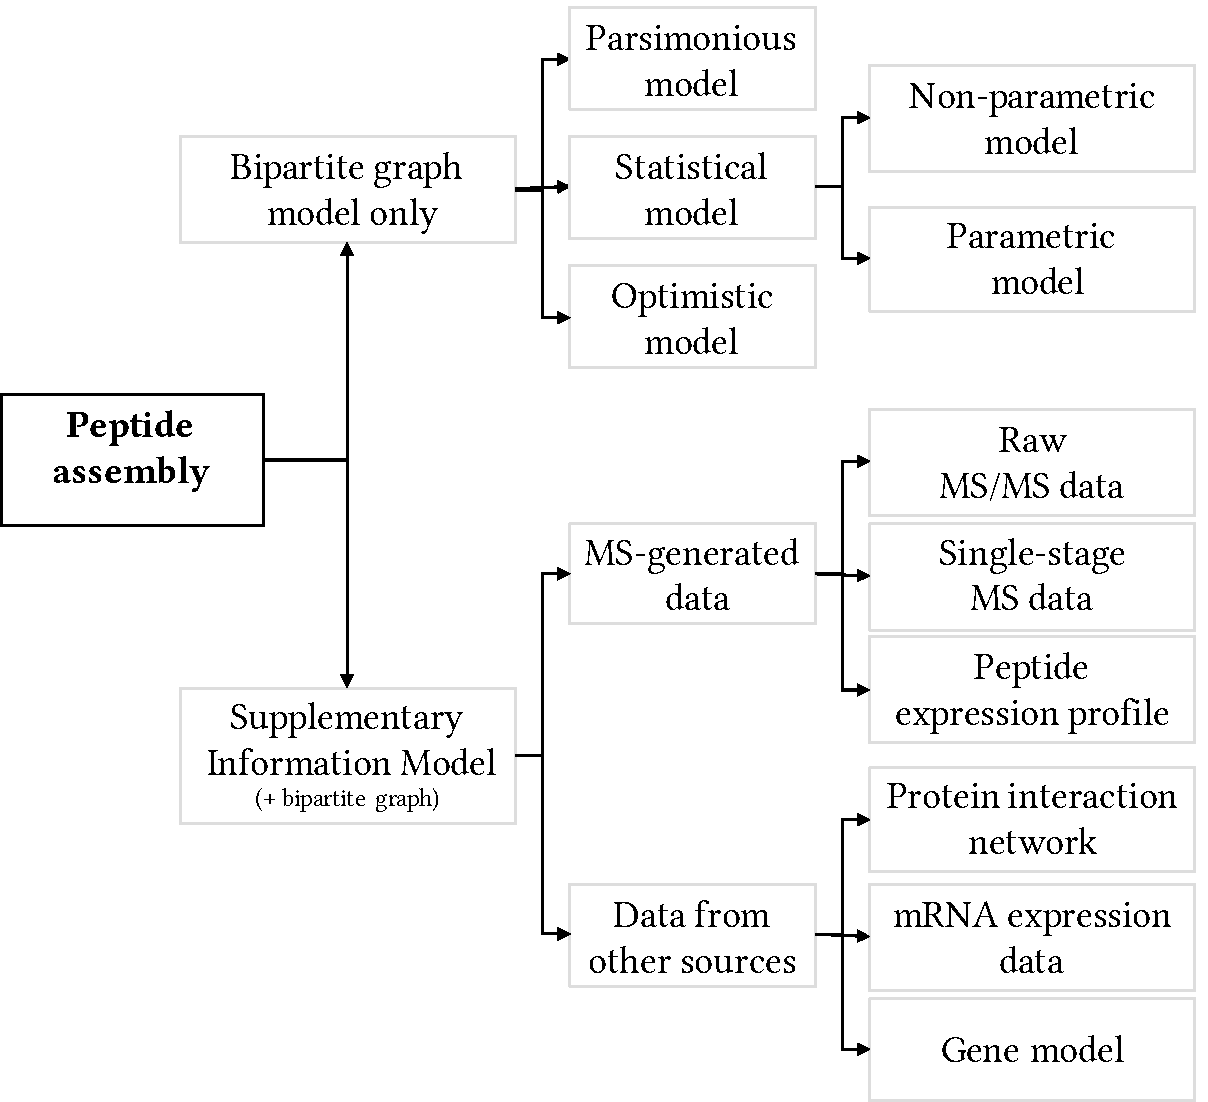
\includegraphics[scale=0.58]{background/ProtInfClass.pdf}\centering
    \caption[Peptide assembly models classification]{\label{fig:ProtInfClass}%
    \textbf{\citet{Huang2012-nr} peptide assembly models classification.}
    }
\end{figure}

\cpv{\citet{Huang2012-nr} describe parametric approaches as
those that request prior knowledge to estimate the peptides' distribution.
When there is no need for prior knowledge,
they describe the approach as non-parametric,
even when the tool assesses the peptide distribution
by extracting information from the \ms\ or \gls{MS/MS} spectra.}\mybr\

\cpv{\section{Bayesian Inference}}\label{app:bayesInf}

\cpv{Bayesian inference is developed upon Bayes' theorem,
which allows the computation of conditional probabilities,
\ie\ computation of the likelihood of an event happening given prior known conditions,
including the likelihood of another event being true.}\mybr\

\cpv{Bayesian statistics focuses on
the credibility of events happening rather than
their occurrence frequencies (as in frequentist statistics).
See \citet{Li2019-ck} for general mathematical definitions of Bayesian inference models
and \citet{Kurt2019-hm} for a layman's guide to Bayesian statistics.}\mybr\

